\documentclass[10pt]{article}
\usepackage{fullpage}
\usepackage{hyperref}
\usepackage{graphicx}
\usepackage{titling}
\usepackage{minted}
\usepackage{enumitem}
\usepackage{dblfloatfix} % For figures at bottom of page

% Progress report (20% Points) (4 pages): 
%
% Propose a model and an algorithm for tackling your task. You should describe
% the model and algorithm in detail and use a concrete example to demonstrate
% how the model and algorithm work. Don't describe methods in general;
% describe precisely how they apply to your problem (what are variables,
% factors, states, etc.)? You should also have finished implementing a
% preliminary version of your algorithm (maybe it's not fully optimized yet
% and it doesn't have all the features you want). Report your initial
% experimental results.

\setlength{\droptitle}{-2cm}

\title{Will I Reply?\\\Large Progress Report}
\author{Anita Lacea (alacea at stanford dot edu)\\Jonathan Wheeler (jamwheel at stanford dot edu)}
\date{\today\\\href{https://github.com/jondoesntgit/willireply}{https://github.com/jondoesntgit/willireply}}

\begin{document}
\maketitle
\begin{figure*}[b]
\begin{center}
$\vcenter{\hbox{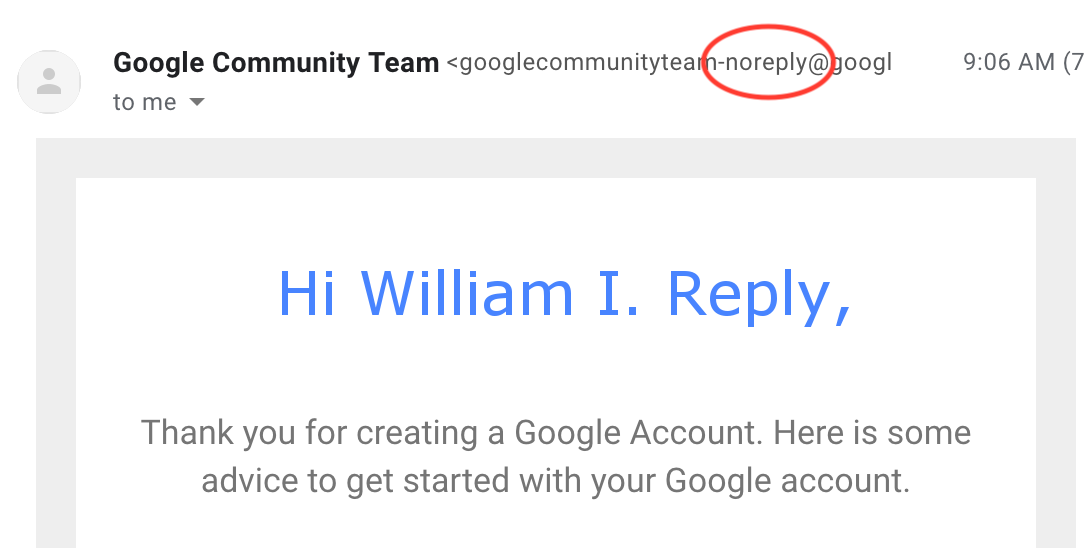
\includegraphics[height=1.5in]{no_reply.png}}} \rightarrow 0 \hspace{3em} 
\vcenter{\hbox{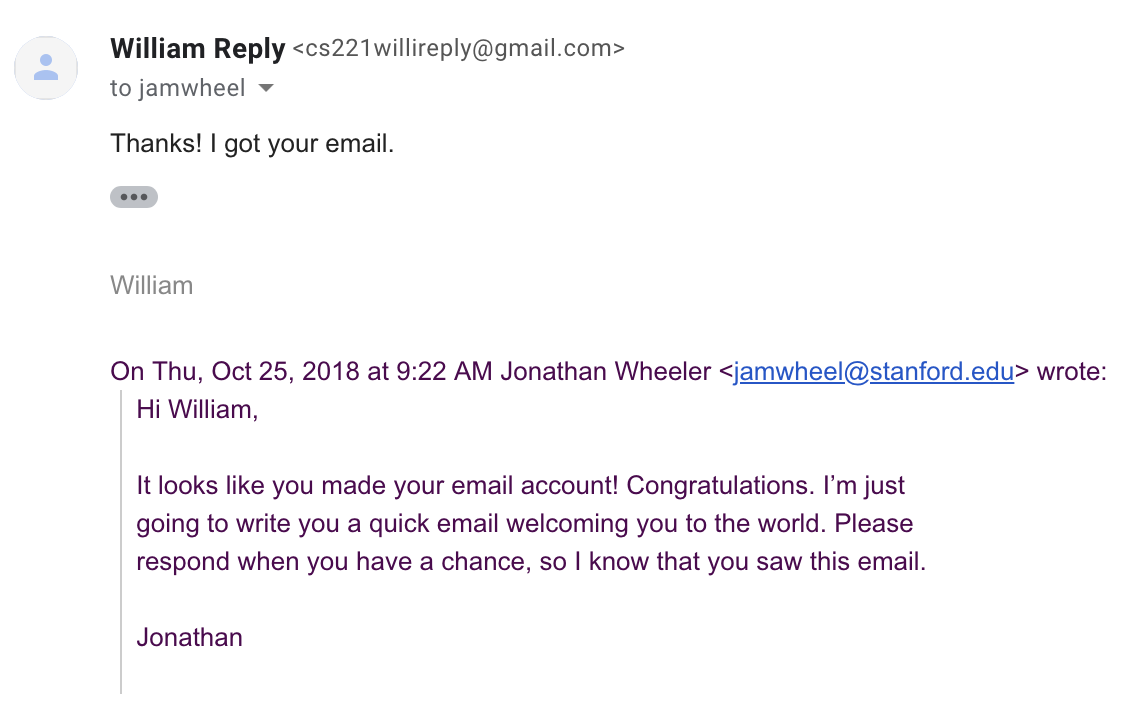
\includegraphics[height=1.5in]{reply_screenshot.png}}} \rightarrow 1 $
\end{center}
\end{figure*}

\section*{Task Definition}

According to one study, business users receive about 140 emails per day, and send about 43 emails per day\cite{emailstatistics}. If we assume that half of the emails that business users send are in response to another email, then only 15\% of emails need a response and the other 85\% are either informational, or require some other action not in the form of an email reply. Work has been done in classifying emails into types calls for papers\cite{learningrulesthatclassifyemail}, spam\cite{filteringjunkemail}, and other so-called ``interesting email''\cite{emailclassification}. Various patents exist disclosing techniques to classify emails\cite{Goodman:2014ug,Bellegarda:2010wk,Romero:2005vs}, and one patent specifically discloses a means of predicting actions (such as replying, forwarding, and deleting) that a user may execute given a new email\cite{Weber:2012tv}.

We propose creating a model that trains on a corpus of emails, and produces a predictor that can classify with high accuracy whether some future email will obtain a response.


\section*{Datasets}

First, we constructed a Python3 script that downloads several hundred to several thousand of a user's most-recent emails from a GMail server. In \texttt{p-proposal}, we demonstrated that a classifier could train on about one hundred emails, and outperform a human oracle who was unfamiliar with my email habits. This experiment was limited in two ways: first, email habits vary substantially from one user to the next, and if the human oracle had the opportunity to view the training set, she would be able to observe certain email habits that deviated from hers, and her performance would likely improve to that of the model or better. Secondly, with only one-hundred training samples, it is possible that the model performed well because of overfitting.

In the last three weeks, we have sought to improve the model by training on a substantially larger dataset. A corpus of about 500,000 emails from 150 distinct users was deemed public domain after the investigation of the Enron Corporation's collapse\cite{enroncorpus}. For each user, there exist between a few tens to several thousands of emails. This dataset allows for a thorough and reproducible investigation to be performed on a static snapshot of the email habits of over one-hundred individuals.

\section*{Preprocessing}

In the case of the GMail dataset, our Python3 script has programatic access to a rich set of metadata about each email. In the first stage of preprocessing, the script extracts each email's body, subject, and headers, and stores these in a sqlite3 database on the local harddrive for rapid indexing. In order to determine what emails obtained a response, the following query is performed:
\begin{minted}{sql}
UPDATE emails SET did_reply = 1
WHERE id in (
  SELECT e_received.id
  FROM emails as e_received
  INNER JOIN emails as e_sent
  WHERE e_sent.reply_id = e_received.message_id
);
\end{minted}
%
where \texttt{message\_id} and \texttt{reply\_id} are values extracted from the GMail headers.

Unfortunately, while the Enron corpus emails contain \texttt{message\_id} headers, the emails do not contain \texttt{reply\_id} header. The absence of \texttt{reply\_id} information in sent emails makes determining what emails were eventually responded to requires more computation.

To label the emails in the Enron corpus, we first take each user, and partition their email folders into two categories: ``sent'' ad ``received'' based on whether they satisfy \texttt{'sent' in folder.lower()}. Then, for each email in a received folder, the labeling script queries on the following conditions:\footnote{This SQL is actually pseudocode. The actual labeling occurs in python, and only the last step is a SQL query.}
\begin{minted}{sql}
UPDATE emails SET did_reply=1
WHERE id IN (
  SELECT e_received.id
  FROM emails as e_received
  INNER JOIN emails as e_sent
  WHERE 'sent' IN e_sent.folder 
  AND 'sent' not IN e_received.folder
  AND e_sent.date > e_received.date
  AND e_sent.subject IN e_received.subject
  AND e_sent.body IN e_received.subject
)
\end{minted}

There are several shortcomings of this algorithm. First, it is very time consuming (takes about one hour to label the 500,000-email corpus). Evaluating the various \texttt{IN} constraints is resource-intensive. Second, there are many scenarios in which a legitimate reply will not be captured by this query. Consider:
\begin{itemize}[noitemsep]
    \item The user responds to an email, and deletes the history in her response
    \item The user responds to an email, but changes the subject line
    \item The user responds to an email, and deletes the file from her sent folder
    \item The user keeps sent emails in folders that do not contain the word `sent'
\end{itemize}

This is a challenge that has been recognized by other investigations of this corpus. Several other methods have been suggested, and we may adapt our labeling script to include these methods\cite{cruzalbrecht:2017,knight:2014}.

The final step of the processing is to detect whether an email is a continuation of a thread, and attempt to split it into it's constituent elements. Currently, this is done by splitting on strings such as \texttt{---Original Message---} or \texttt{On 11/15/2001, email@example.com wrote}.

\section*{Features}

We are interested in training a model to produce a predictor that can predict whether an email will be replied to based on the properties of that email. There are two classes of features that can be assigned to each email. The first class of features are general enough that they can be applied to any email, regardless of the user. Some of these features include

\begin{itemize}[noitemsep]
\item Number of users in \texttt{To:}
\item Number of users in \texttt{Cc:}
\item Number of question marks in subject, or in body
\item Number of keywords in the email body or header (such as `please', `asap')
\item Whether the email was forwarded or replied to (indicated by the first word in the subject)
\item The number of prior messages in the thread
\item Number of words in subject or body
\end{itemize}

Other features that are present in other works on the Enron corpus include presence of attachments, presence of links, and a TF-IDF of the body or subject. \cite{cruzalbrecht:2017,knight:2014,bromberg:2013}

The second class of features are more unique to a user, and require greater knowledge about this user's specific history or persona:

\begin{itemize}[noitemsep]
\item Is this email from a sender the user frequently responds to?
\item Is this email CCed to the user, or is it TO the user?
\item Is this user's first name (or last name with a salutation) in the email? Are other user's names also present?
\item How frequently does the user receive email from this sender?
\end{itemize}

While these features grant the model a richer picture of the background of the email, the weights associated with these features do not easily transfer from one user to the next (some users may go by nicknames, some users are managers while others are sales, while others may be developers). 

\section*{Model}

Thus far, we have implemented a stochastic-gradient-descent (SGD) regressor using various combinations of the universal features. In our prelinary tests, we have trained the model on the emails of a few tens of users (representing tens of thousands of emails), and validated the model on a user that was not part of the training set. 

\section*{Evaluation}

Binary classifiers are often characterized by their `precision' and `recall' parameters. In our case, the precision of the `reply' label will tell us how often a prediction that we would reply to an email was correct, and the recall of the `reply' label will tell us what percentage of the emails that require a response are correctly being identified. Because the majority of email that most users received is often requires no action (spam, informational, etc...), the precision and recall of the `no reply' label will always be quite high, and we are not interested in optimizing these parameters.

Recall and precision are both important, and so our metric will include a component of both, but the reply recall is more important for our algorithm. Failing to capture an email that requires a response (recall) is more critical than the inconvenience of being exposed to an email that requires no response (precision). In this case, we might use an $F_\beta$ metric\cite{fbetawikipedia}. For $\beta = 1$, precision and recall are weighted equally. For $\beta > 1$, recall is weighted more heavily. We arbitrarily set $\beta = 2$, to make recall twice as important as precision. This is the overall metric that we use to evaluate our performance. $F_2 = 0$ is the worst case scenario, $F_2 = 1$ is the best case scenario.

The figure of 

\section*{Experimental Results}

Across a majority of the tests that we have done, we have achieved an $F_2$-value of about 17\%. In our initial testing, a human oracle labeled 200 of Jonathan's emails, and achieved a $F_2$-value of 15.5\%. So these models we have developed thus far on the Enron corpus seem to perform somewhat better than a human oracle. 

However, 17\% is not significant enough to rely on this algorithm in practice to capture important emails. We can reference other works that have sought to classify emails based on their likelyhood to respond. \cite{knight:2014} was able to achieve $F_1$ scores of about 40-50\% when training and validating on the same personal email account. \cite{bromberg:2013} report the recall and precision for training and recall on a personal email account, which can be converted into an $F_{\beta = 2}$ score via
$$
F_\beta = (1+\beta^2)\frac{\mathrm{precision} \cdot \mathrm{recall}}{\beta^2 \cdot \mathrm{precision} + \mathrm{recall}}.
$$

Using a na\"ive Bayes model, they achieved an $F_2$ value of 0.26 using similar features to those presented here. Using a support vector machine (SVM) model, they were able to achieve an $F_2$ value of 0.60 (precision: 37.64\%,
recall: 71.33\%). While these results are much better than our results, their algorithm had the luxury of training and testing on the same user, whereas ours trains on one user and tests on another. For comparison, when we do a similar test using only a feature that extracts whether the user responded to the sender in the past, our linear model achieves an $F_2$ of 42\%.

\section*{Challenges}

There are several challenges we are continuing to improve upon. 

First, email software varies from user to user in the way that they handle threads and replies. And because every email conversation is going to involve two users using two different computers with possibly different email softwares, writing parsers to determine what constitutes a reply or a thread is challenging. Thankfully, the headers in the Enron corpus are more-or-less standard, yet they lack the \texttt{reply\_to} header that would make tagging replies easier. However, even users at the same corporation will have different habits. Some users will delete archived email threads, stuff (or duplicate) emails across multiple folders. Tracking these changes has proven somewhat difficult.

Furthermore, every user has different email habits. Some users sign up to more marketing, and others keep their inboxes sparse. Some users prefer to use email for all communication, while other users may only use it for certain applications like business with external colleagues. Because each user's style is different, it is difficult to generalize a fit from user A's history to predict how user B will behave. Users themselves may change habits over time, so a fit from an Enron employee in 2001 may not accurately predict their email habits in 2018.

In the upcoming weeks, we will be fine-tuning our model (possibly entertaining different loss functions, etc...), and adjusting some of our features to improve our $F_2$ score.

\bibliography{../bibliography} 
\bibliographystyle{ieeetr}

\end{document}
